
\begin{center}

\includegraphics[width=0.4\textwidth]{content/3/chapter4/images/31.png}\\
Cippi接受了神圣的触摸
\end{center}

指定初始化是聚合初始化的特例。

\subsubsubsection{4.4.1\hspace{0.2cm}聚合初始化}

首先:什么是聚合?聚合是数组和类型。类型可以是一个类、一个结构体或一个联合体。

C++20中,支持聚合初始化的类型必须满足以下条件:

\begin{itemize}
\item 
没有private或protected的非静态数据成员

\item 
没有用户声明的或继承的构造函数

\item 
没有虚基类、private基类或protected基类

\item 
没有虚成员函数
\end{itemize}

下面的程序演示了聚合初始化。

\begin{lstlisting}[style=styleCXX]
// aggregateInitialization.cpp

#include <iostream>

struct Point2D{
	int x;
	int y;
};

class Point3D{
public:
	int x;
	int y;
	int z;
};

int main(){

std::cout << '\n';

	Point2D point2D{1, 2};
	Point3D point3D{1, 2, 3};
	
	std::cout << "point2D: " << point2D.x << " " << point2D.y << '\n';
	std::cout << "point3D: " << point3D.x << " " << point3D.y << " "
							 << point3D.z << '\n';
	
	std::cout << '\n';

}
\end{lstlisting}

第21和22行使用大括号直接初始化聚合,大括号中的初始化式的顺序必须与成员的声明顺序匹配。介绍三向比较操作符的部分中,有挺复杂的聚合初始化示例。

\begin{center}
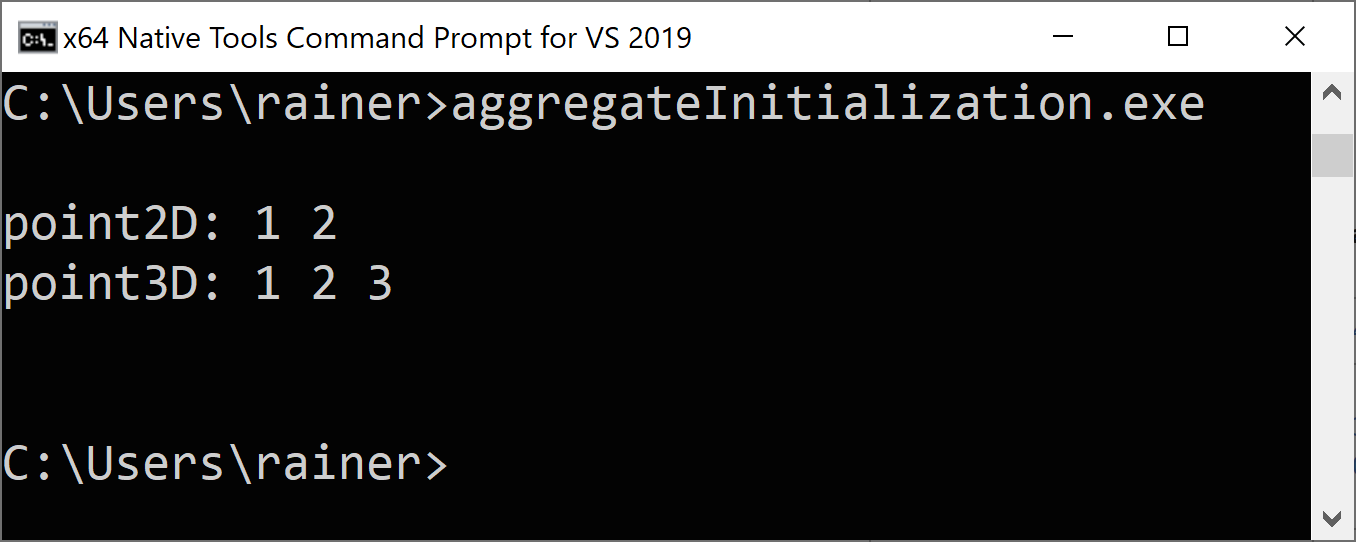
\includegraphics[width=0.6\textwidth]{content/3/chapter4/images/32.png}\\
\end{center}

基于C++11中的聚合初始化,C++20出现了设计好的初始化器。到2020年底,只有Microsoft编译器完全支持指定初始化。

\subsubsubsection{4.4.2\hspace{0.2cm}类成员的命名初始化}

指定初始化允许使用类型成员名直接初始化。对于联合体,只能提供一个初始化式。对于聚合初始化,大括号中的初始化式的顺序必须与成员的声明顺序匹配。

\begin{lstlisting}[style=styleCXX]
// designatedInitializer.cpp

#include <iostream>

struct Point2D{
	int x;
	int y;
};

class Point3D{
public:
	int x;
	int y;
	int z;
};

int main(){
	
	std::cout << '\n';
	
	Point2D point2D{.x = 1, .y = 2};
	Point3D point3D{.x = 1, .y = 2, .z = 3};
	
	std::cout << "point2D: " << point2D.x << " " << point2D.y << '\n';
	std::cout << "point3D: " << point3D.x << " " << point3D.y << " "
							 << point3D.z << '\n';
	
	std::cout << '\n';
	
}
\end{lstlisting}

第21和22行使用指定的初始化器来初始化聚合,像.x或.y这样的初始化式称为指示符。

\begin{center}
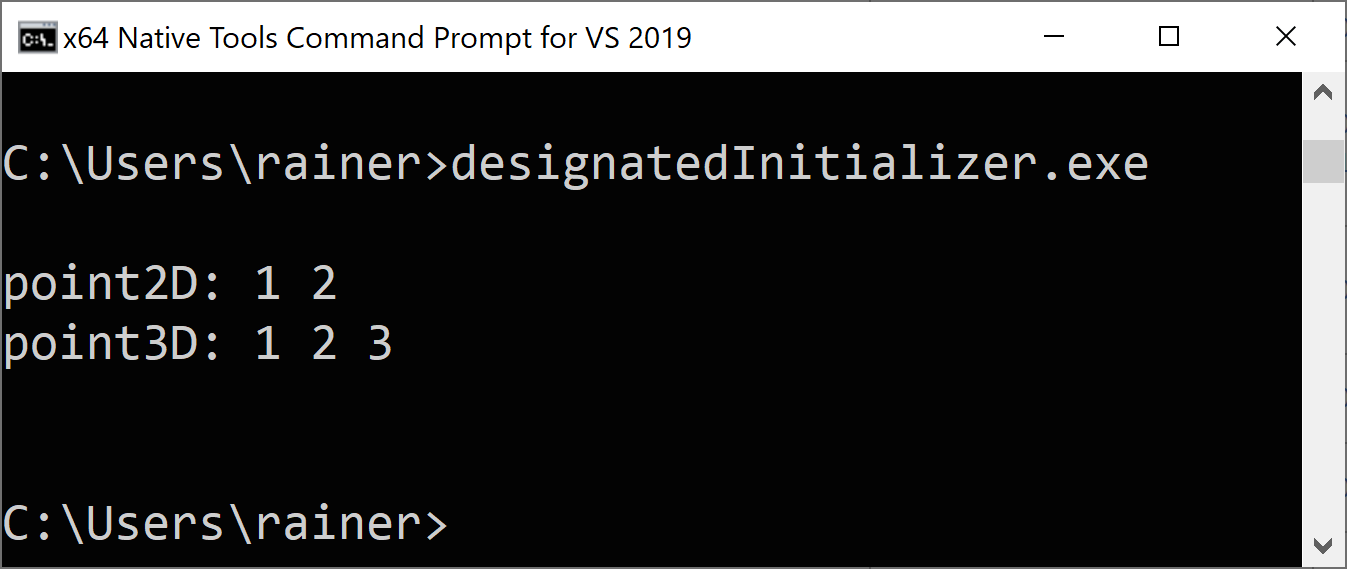
\includegraphics[width=0.6\textwidth]{content/3/chapter4/images/33.png}\\
\end{center}

聚合成员可以已经有默认值,当缺少初始化式时使用此默认值,但这并不适用于联合体。

\begin{lstlisting}[style=styleCXX]
// designatedInitializersDefaults.cpp

#include <iostream>

class Point3D{
public:
	int x;
	int y = 1;
	int z = 2;
};

void needPoint(Point3D p) {
	std::cout << "p: " << p.x << " " << p.y << " " << p.z << '\n';
}

int main(){
	
	std::cout << '\n';
	
	Point3D point1{.x = 0, .y = 1, .z = 2}
	
	std::cout << "point1: " << point3D.x << " " << point3D.y << " "
							<< point3D.z << '\n';
							 
	Point3D point2;		 
	std::cout << "point2: " << point2.x << " " << point2.y << " "
							<< point2.z << '\n';
				
    Point3D point3{.x = 0, .z = 20};			 
	std::cout << "point3: " << point3.x << " " << point3.y << " "
							<< point3.z << '\n';
	
	// Point3D point4{.z = 20, .y = 1}; ERROR
	
	needPoint({.x = 0});
	
	std::cout << '\n';
	
}
\end{lstlisting}

第20行初始化了所有成员,但第24行没有为成员x提供值,x没有初始化。若只初始化没有默认值的成员,比如在第28行或第34行中没问题,因为z和y的顺序是错误的,第32行中的表达式则无法编译。

\begin{center}
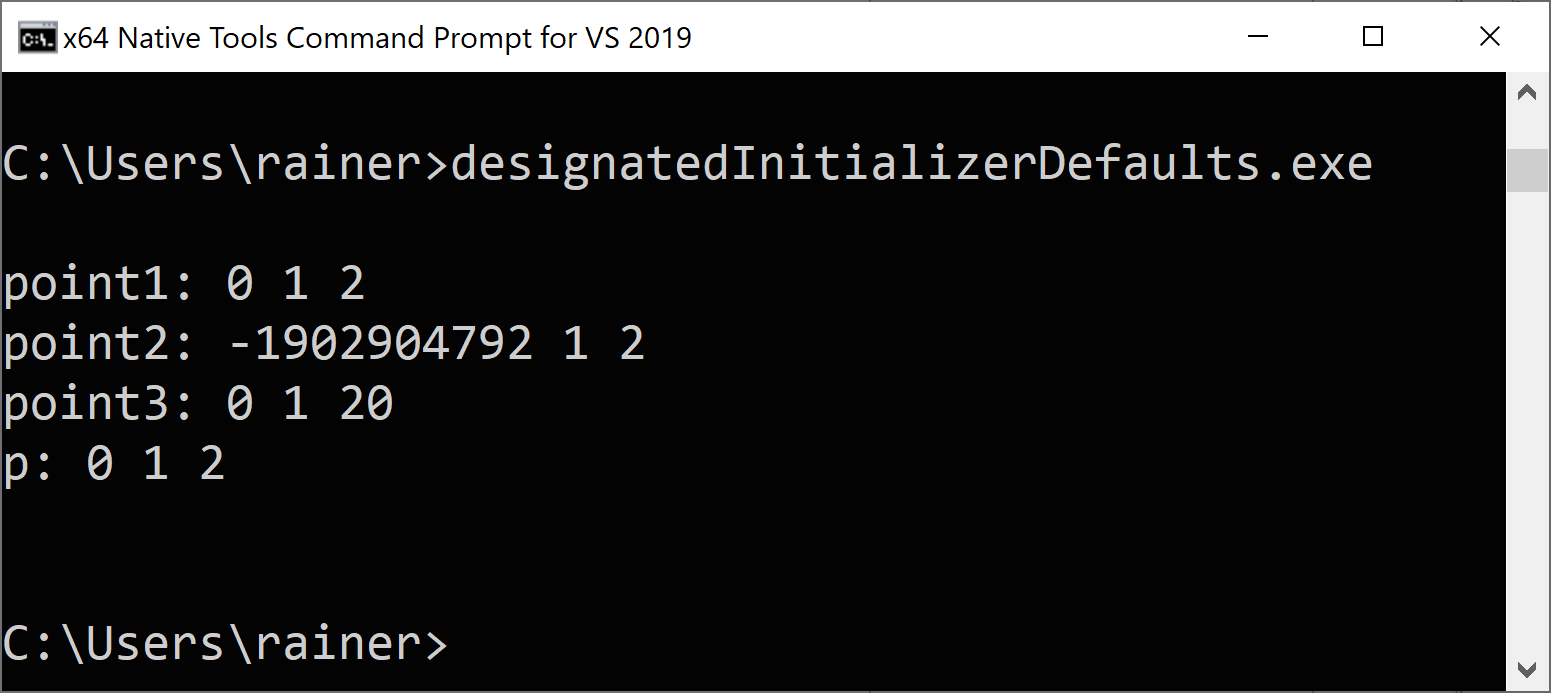
\includegraphics[width=0.6\textwidth]{content/3/chapter4/images/34.png}\\
\end{center}

指定初始化器检测窄化转换,导致精度降低。

\begin{lstlisting}[style=styleCXX]
// designatedInitializerNarrowingConversion.cpp

#include <iostream>

struct Point2D{
	int x;
	int y;
};

 class Point3D{
public:
	int x;
	int y;
	int z;
};

int main(){
	
	std::cout << '\n';
	
	Point2D point2D{.x = 1, .y = 2.5};
	Point3D point3D{.x = 1, .y = 2, .z = 3.5f};
	
	std::cout << "point2D: " << point2D.x << " " << point2D.y << '\n';
	std::cout << "point3D: " << point3D.x << " " << point3D.y << " "
							 << point3D.z << '\n';
	
	std::cout << '\n';

}
\end{lstlisting}

因为初始化.y = 2.5和.z = 3.5f会窄化为int,所以第21行和第22行会产生编译时错误。

\begin{center}
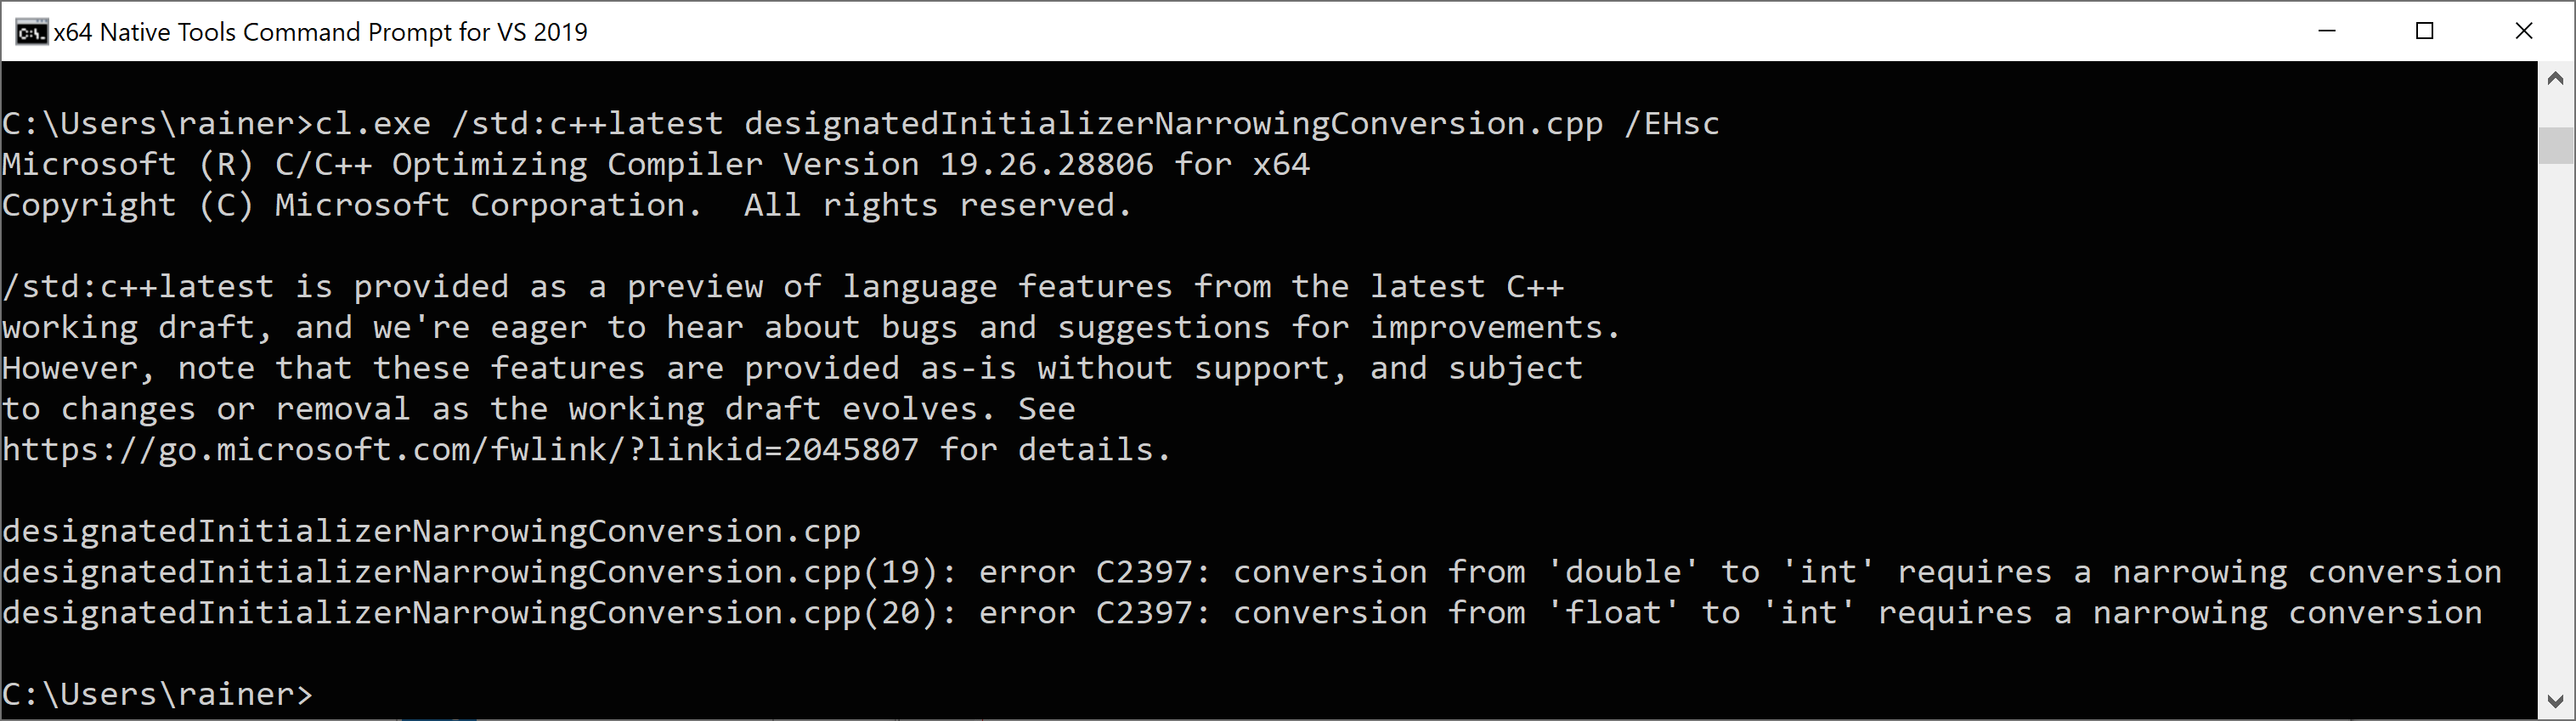
\includegraphics[width=1.0\textwidth]{content/3/chapter4/images/35.png}\\
\end{center}

有趣的是,指定初始化式在C和C++的行为不太一样。

\begin{tcolorbox}[breakable,enhanced jigsaw,colback=red!5!white,colframe=red!75!black,title={C和C++的区别}]
C指定的初始化器支持C++中不支持的用例。

C允许:

\begin{itemize}
\item 
乱序初始化聚合的成员

\item 
初始化嵌套聚合的成员

\item 
混合指定初始化式和常规初始化式

\item 
数组的指定初始化
\end{itemize}

提案\href{http://www.open-std.org/jtc1/sc22/wg21/docs/papers/2017/p0329r4.pdf}{P0329R4}为这些用例提供了示例:

\begin{lstlisting}[style=styleCXX]
struct A { int x, y; };
struct B { struct A a; };
struct A a = {.y = 1, .x = 2}; // valid C, invalid C++ (out of order)
int arr[3] = {[1] = 5}; // valid C, invalid C++ (array)
struct B b = {.a.x = 0}; // valid C, invalid C++ (nested)
struct A a = {.x = 1, 2}; // valid C, invalid C++ (mixed)
\end{lstlisting}

C和C++这种差异的原理,也是提案的一部分:“C++成员以反向构造顺序销毁,初始化式列表的元素以词法顺序求值,因此字段初始化式必须按顺序指定。数组指示符与Lambda表达式语法冲突。嵌套的指示符则很少使用。”提案还认为,只有乱序初始化聚合会经常使用。

\end{tcolorbox}	

\begin{tcolorbox}[breakable,enhanced jigsaw,colback=mygreen!5!white,colframe=mygreen!75!black,title={总结}]
指定初始化是聚合初始化的一种特殊情况,使其能够使用类成员名初始化类成员。初始化顺序必须与声明顺序匹配。
\end{tcolorbox}	

\newpage






